%%
%% Author: Dario Chinelli
%% begin 2019-12-04
%% last mod 2022-02-02
%%

% Preamble
\documentclass[class=article, crop=false]{standalone}

% Packages
\usepackage[subpreambles=true]{standalone}
\usepackage{import}
\usepackage{graphicx}
\usepackage{amsmath}

% Document
\begin{document}

% Simulations documentation here


\FloatBarrier
\paragraph{Probability distribution}
The tool used here to get a move probability is a tensor.
For each position, and eventually time, it returns a number between $0$ and $1$.
The sum over every directions is $1$, because of the normalization.
This tensor is multidimensional, as described in the previous paragraphs, and its dimension depends on the model.
With this tool is possible to plot the map with the corresponding probability for each of the nine directions.
It is possible to see along the trajectories where is the more probable direction to take and which is the less.
To describe this lets take into account just a few real trajectories, with a common path and and opposite directions.
So are considered five pedestrians in (Figure \ref{fig:5pids_trjl}), with two representations:
one plotting the actual lines in the field (Figure \ref{fig:5pids_trjlines}) and one adding in a heat-map where pedestrians passed through (Figure \ref{fig:5pids_trjlhist}).
\begin{figure}[h]
    \centering
    \subfloat[Trajectories lines of five "real" pedestrians.]{
        \label{fig:5pids_trjlines}
        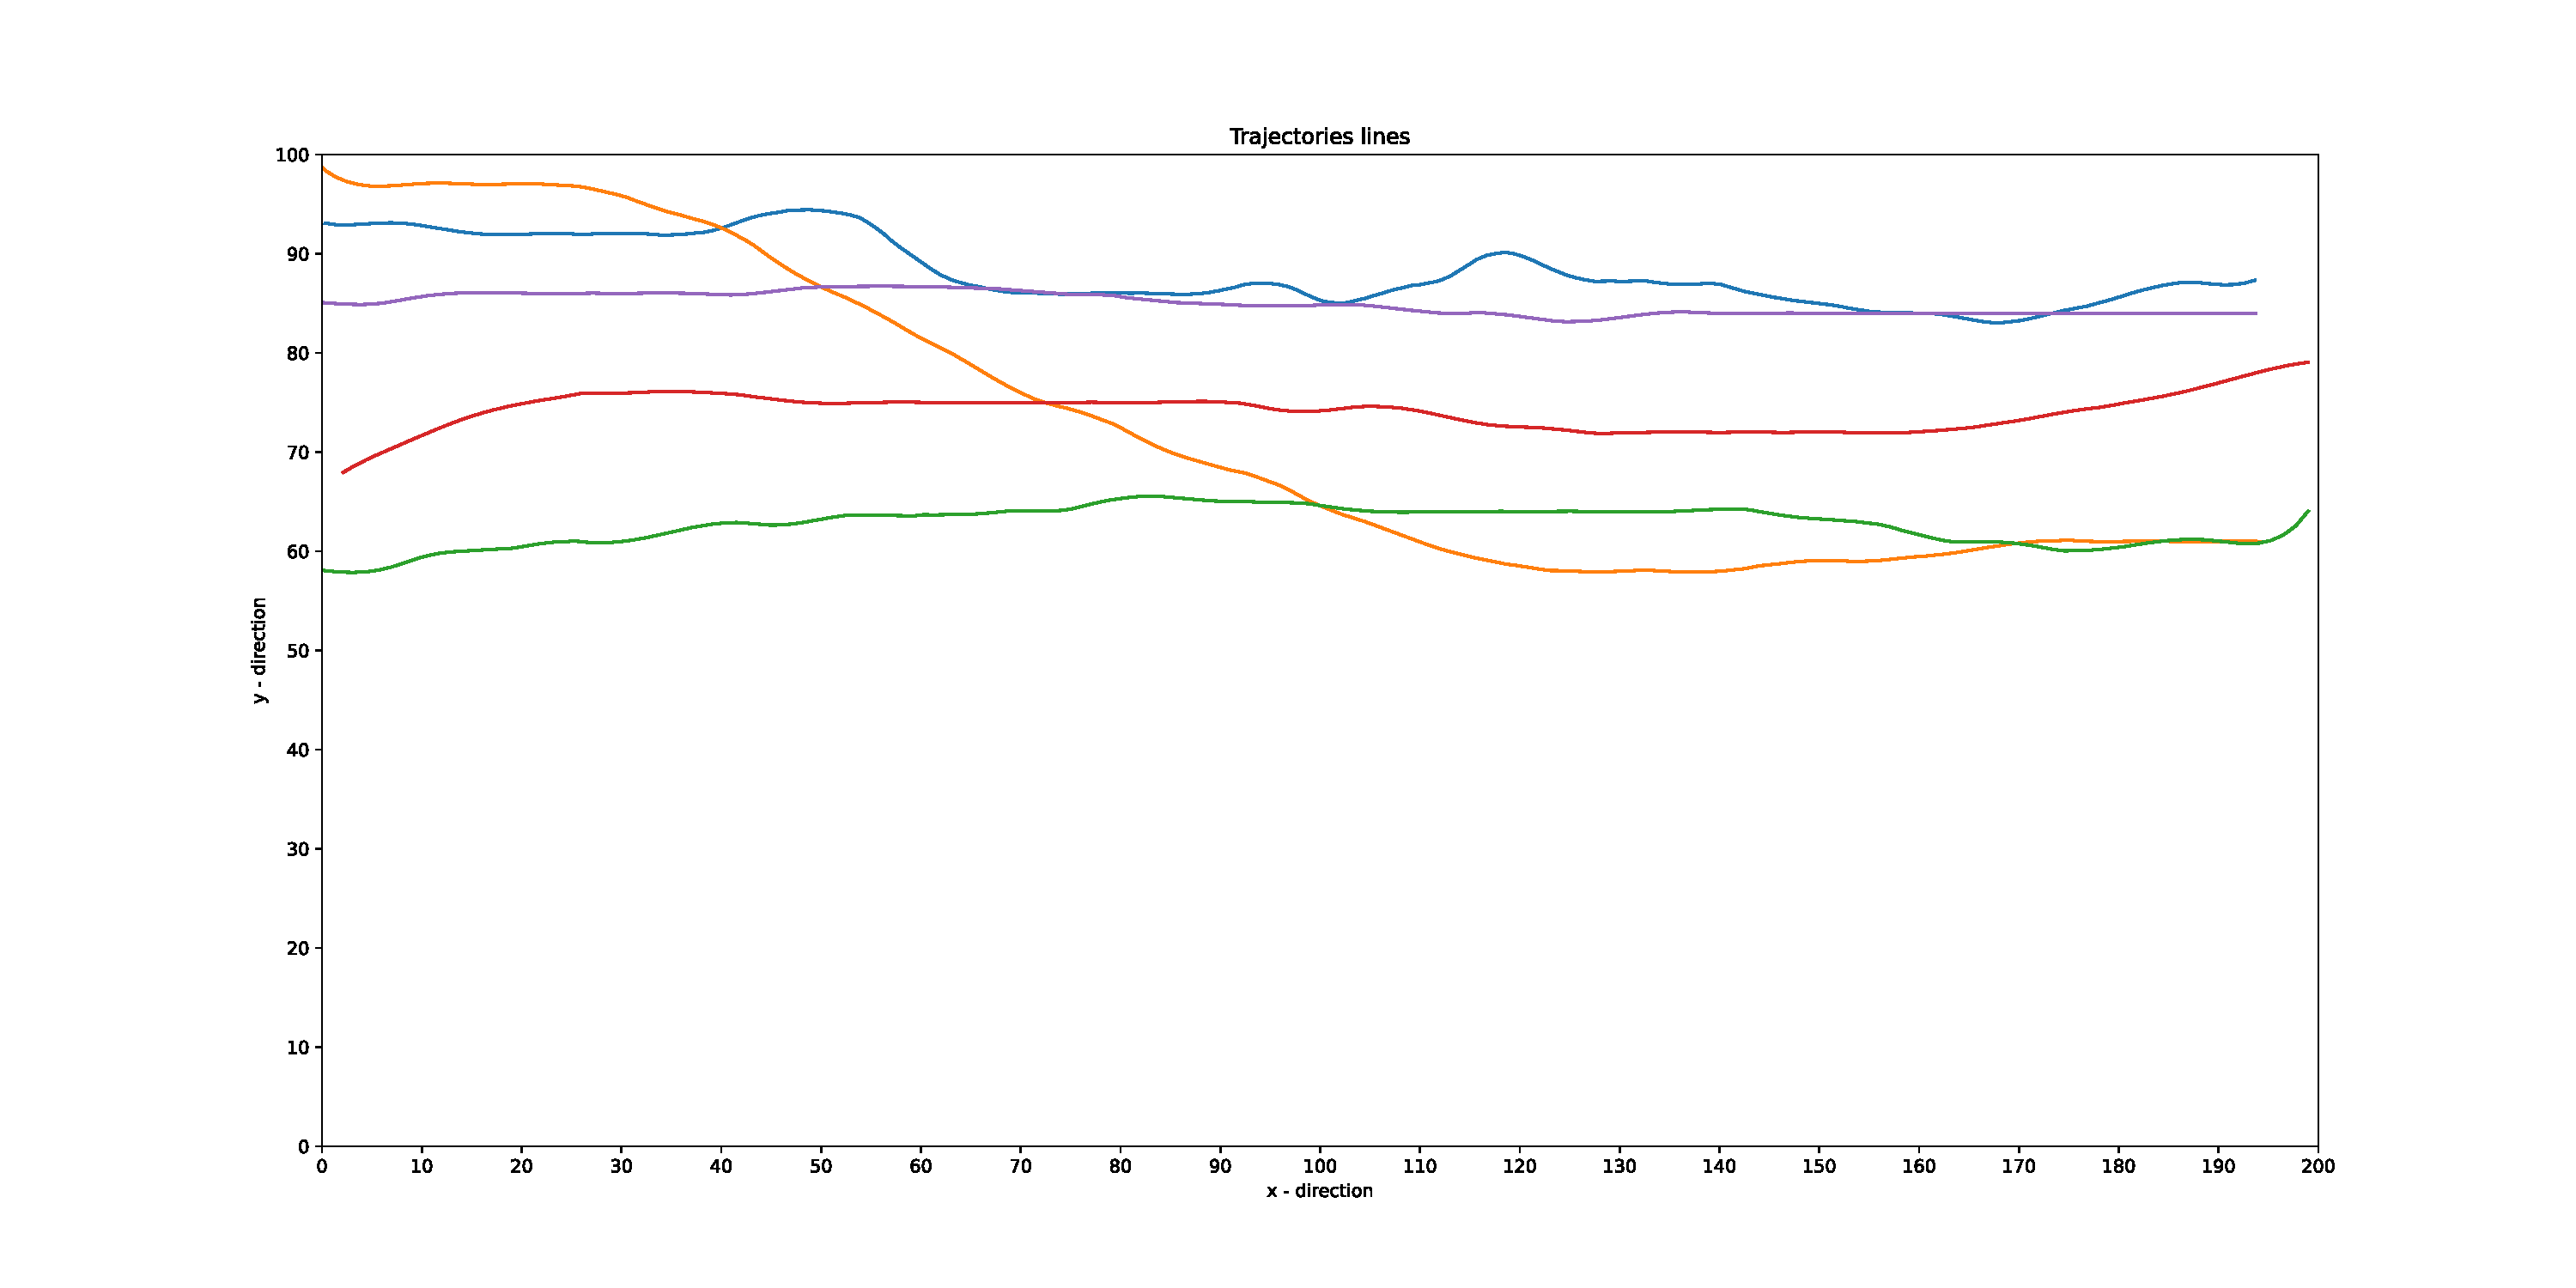
\includegraphics[ width=0.45\textwidth]{fig/5pids/figure_trainf10_few_trajectories_Dx200_Dy100_TRJLINES}
    }\quad
    \subfloat[Trajectories heatmap of five "real" pedestrians.]{
        \label{fig:5pids_trjlhist}
        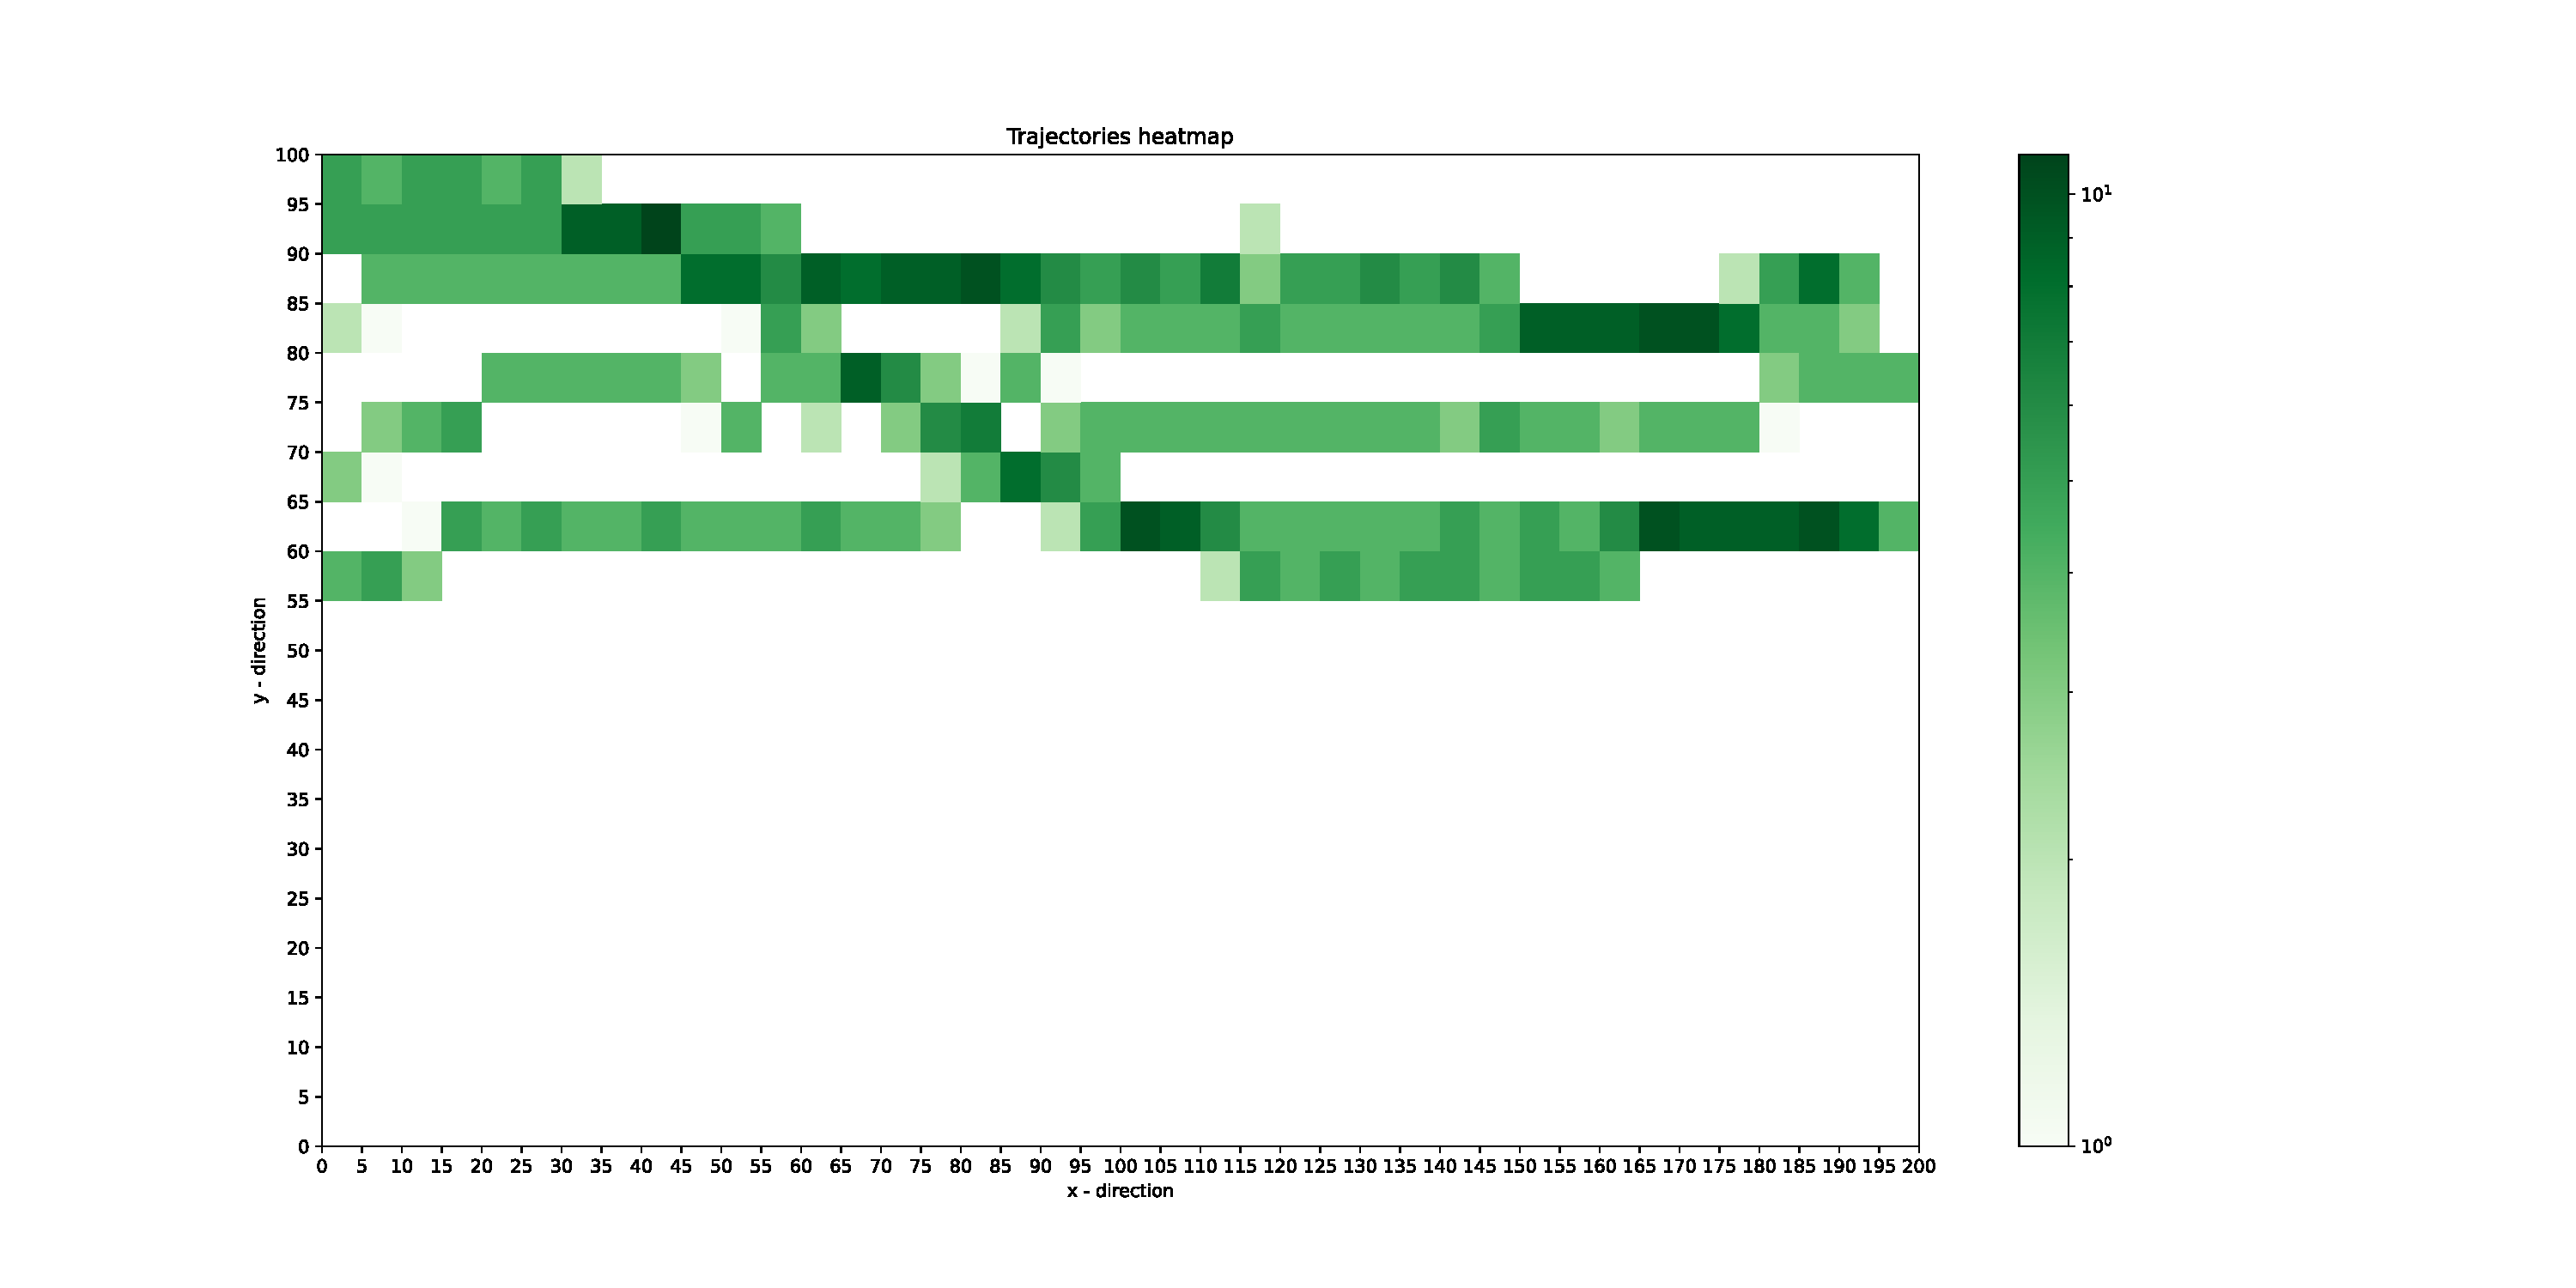
\includegraphics[ width=0.4\textwidth]{fig/5pids/figure_trainf10_few_trajectories_Dx200_Dy100_TRJHIST}
    }
    \captionsetup{width=.8\linewidth}
    \caption{Representation of five real trajectories from dataset.}
    \label{fig:5pids_trjl}
\end{figure}
\paragraph{Velocities plot}
An useful plot to understand those paths is the one that compare the velocity along the two axes $x$ and $y$.
In this example it describes how some trajectories are going left and others are walking right, see the (Figure \ref{fig:5pids_velhist}).
\begin{figure}[h]
\centering
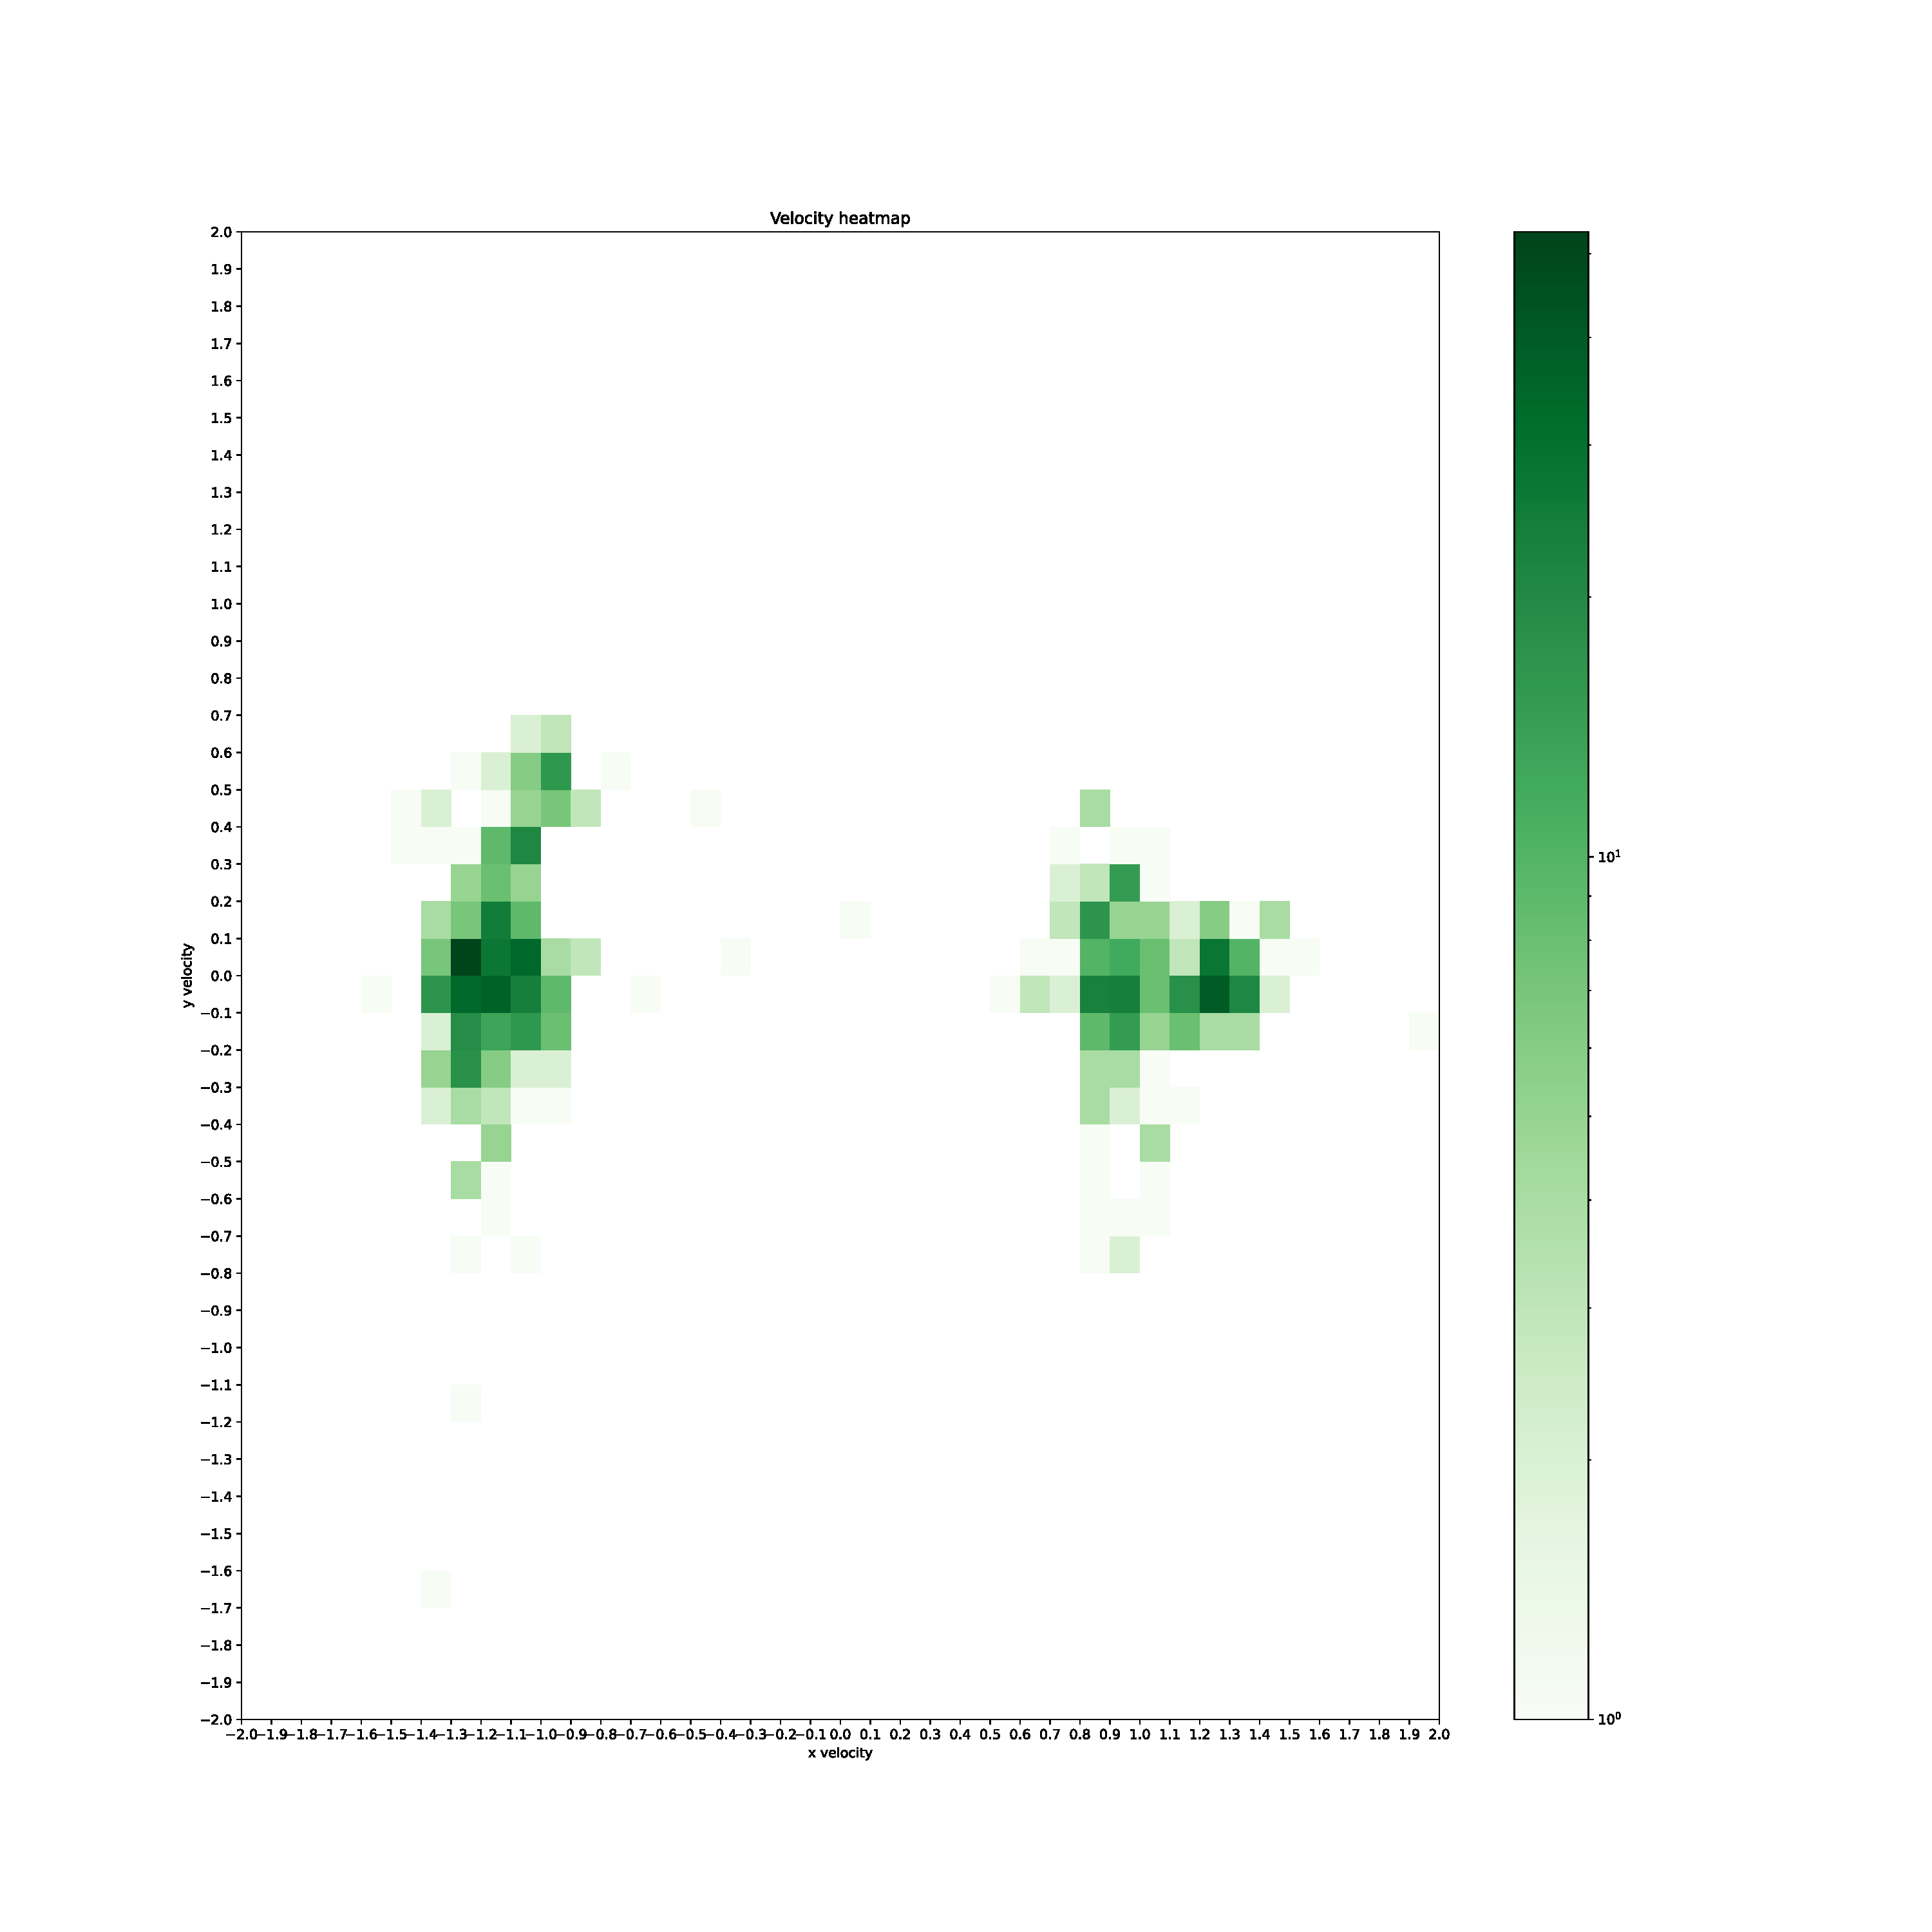
\includegraphics[scale=0.1]{fig/5pids/figure_trainf10_few_trajectories_Dx200_Dy100_VELHIST}
\captionsetup{width=.5\linewidth}
\caption{Comparison between velocity along the two directions $v_x$ and $v_y$.}
\label{fig:5pids_velhist}
\end{figure}
\paragraph{D2Q9 representation}
With this introduction is now possible to look at the $3\times3$ matrix plot that follows.
The plot in (Figure \ref{fig:5pids_D2Q9}) is composed by nine plots.
In each of those is plotted the move probability in just one direction and it is oriented as the usual $D2Q9$ map that is showed before in (Figure \ref{fig:D2Q9_k}).
So that the center figure represents the probability to stand still, meanwhile the right-center figure is the probability to move right and so on.
\begin{figure}[h]
\centering
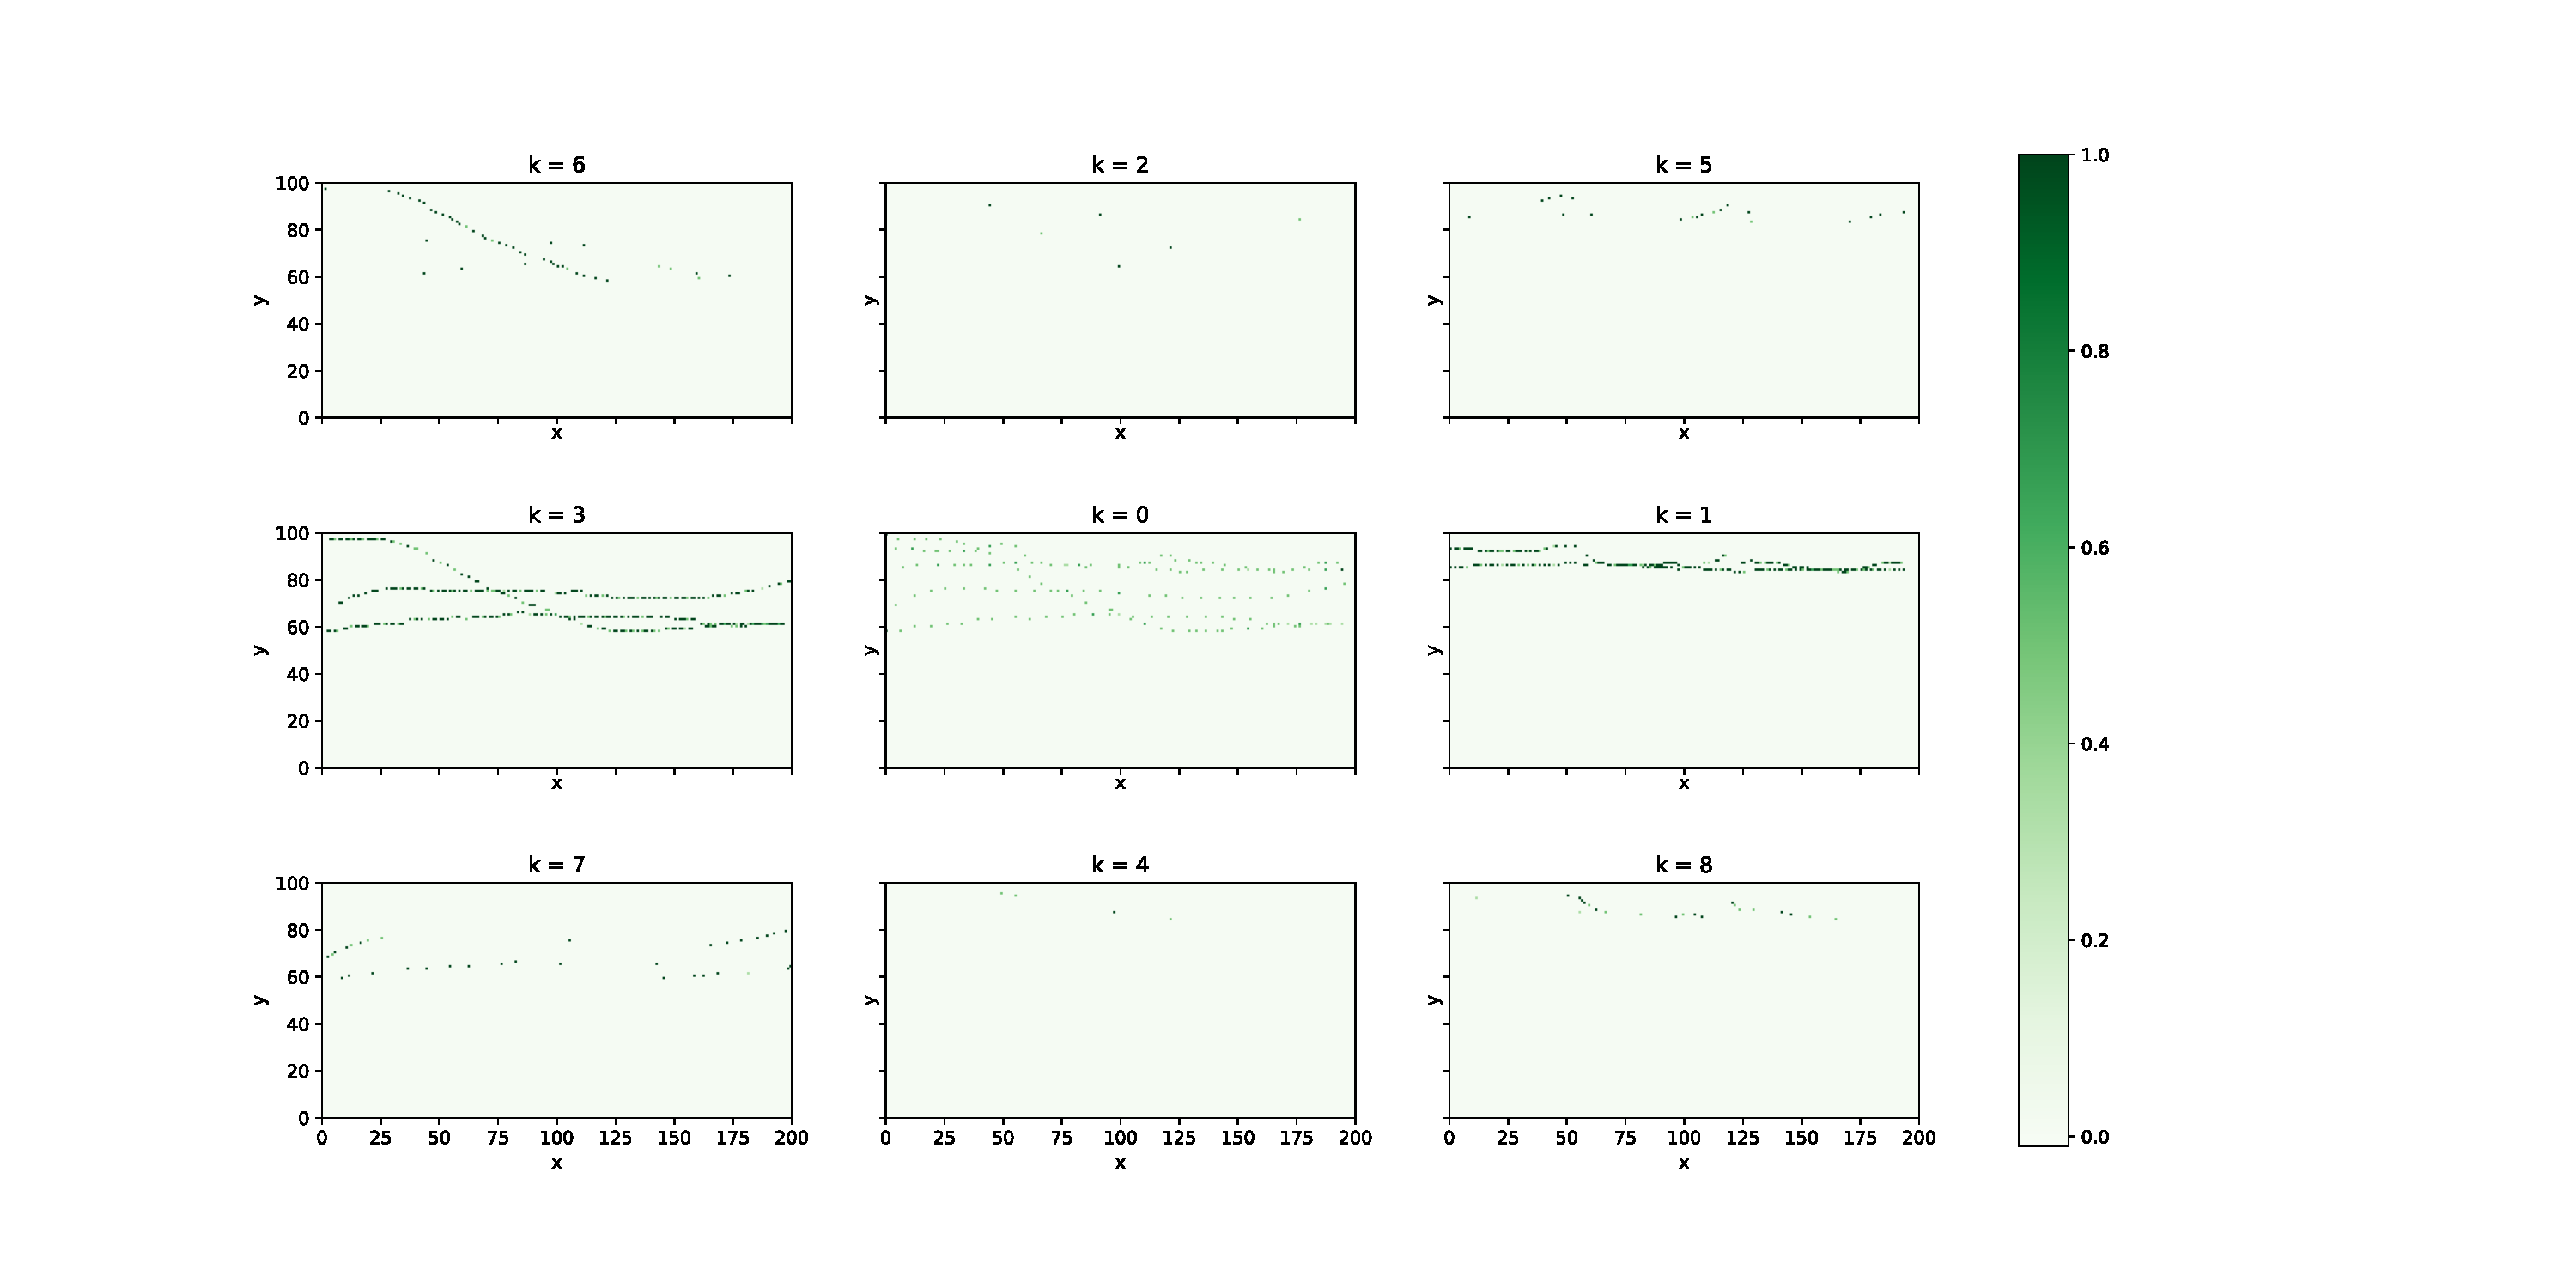
\includegraphics[scale=0.25]{fig/5pids/figure_trainf10_few_trajectories_Dx200_Dy100_D2Q9}
\captionsetup{width=.6\linewidth}
\caption{Representation of the D2Q9 model. Every plot shows the move probability for each associated direction.}
\label{fig:5pids_D2Q9}
\end{figure}




\FloatBarrier
\subsection{Trajectories simulation}


\FloatBarrier
\subsection{Distribution simulation}


\end{document}
